\vspace{10pt}

{\centering\subsection*{龙柏泉:如何写好一个故事?}}

\addcontentsline{toc}{subsection}{龙柏泉:如何写好一个故事?}

\renewcommand{\leftmark}{龙柏泉:如何写好一个故事?}

\begin{figure}[htbp]

\centering

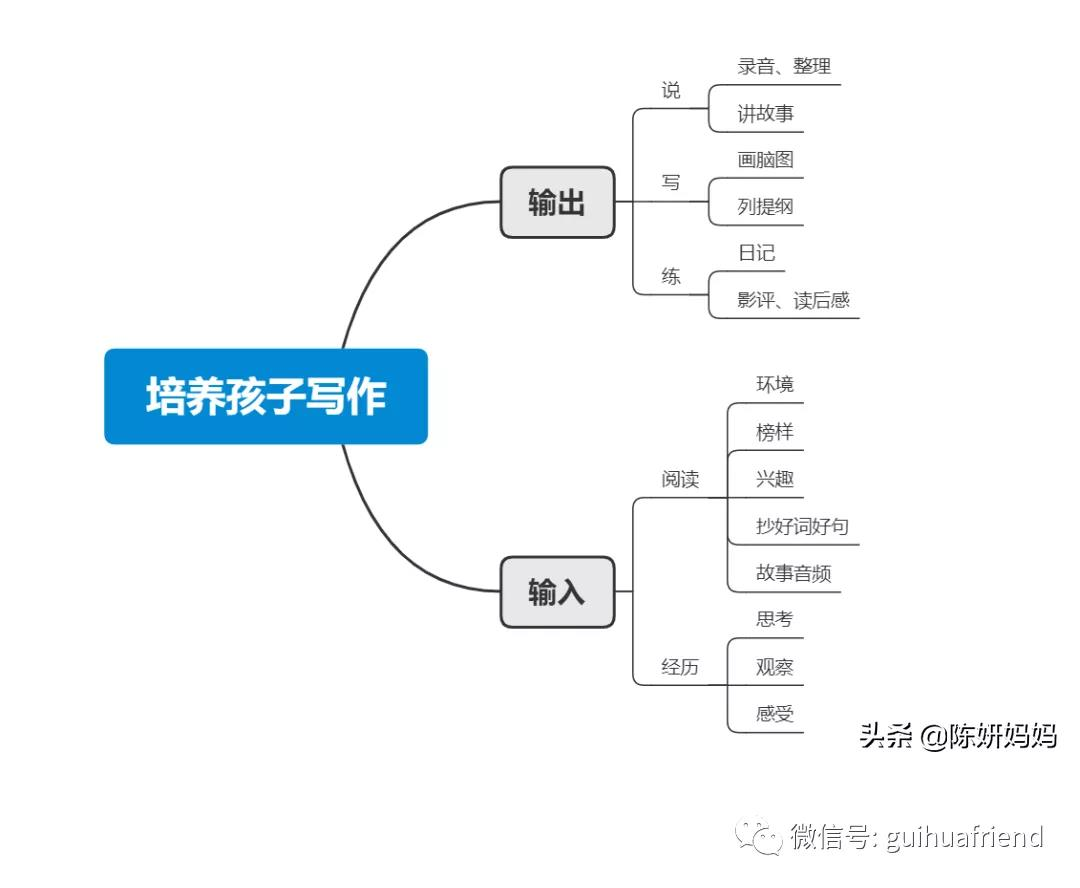
\includegraphics[width = .5\textwidth]{./ch/v6.jpg}

\end{figure}

与你共同成长。



你好,这里是桂花图书馆阅读分享,我是馆长莫静琴。



上一周周璇老师分享了“如何描写人物”,这一周我们想分享“如何写好一个故事”。



关于如何写一个故事,我相信每个人的中小学时代,语文老师都给我们做了充分的指导和练习。例如记叙文的六要素,即故事的时间、地点和人物,故事的起因、经过和结果。基本上,写好一个故事,或者阅读后分析清楚一个故事的这些要素,锻炼的是孩子结构化思维的能力,和对复杂的系统进行梳理的能力。





在这里我也谈一谈对于小学生如何写好一个故事的想法。



第一点,建议写亲身经历的事。自己亲身经历的故事,更容易动笔,有更加合理的情节,更加丰富的内容,更加真切的感受。这样的故事写出来,会更真实感人,更容易让读者产生共鸣。即便是很多想象的故事情节,也可以参考生活的经历来组织。



第二点,从小故事写起。小故事情节更加简单,小学生更容易驾驭或者是掌控。小故事包含细节,也往往可以以小见大。小故事往往需要细致的观察,清晰的回忆,丰富的联想,精准的词汇。把一个小故事细致入微的叙述出来,能够锻炼自己的思维和文笔。



第三点,动笔之前可以先把故事讲给身边的人听。身边的人在听故事的过程中,会提出自己没听懂的,或者感兴趣的地方。对于这些地方的补充和反馈,会让故事逻辑更加合理,细节更加丰满。



最后,可以先按故事的要素构思简单的故事框架。例如画图,或者用简单的文字把关键要素写出来,列个提纲。然后根据提纲,丰富具体的细节,这样写作起来会更有方向感,更有条理。







以上便是我的一些想法,谢谢大家!

\vspace{10pt}

文稿:龙柏泉

朗读:莫静琴

发布:2021年5月16日








\vspace{10pt}

\hline

